\documentclass[a4paper,11pt]{article}

% Kodovani (cestiny) v dokumentu: utf-8
%\usepackage[cp1250]{inputenc}	% Omezena stredoevropska kodova stranka, pouze MSW.
\usepackage[utf8]{inputenc}	% Doporucujeme pouzivat UTF-8 (unicode).

\usepackage[margin=2cm]{geometry}
\newtoks\jmenopraktika \newtoks\jmeno \newtoks\datum
\newtoks\obor \newtoks\skupina \newtoks\rocnik \newtoks\semestr
\newtoks\cisloulohy \newtoks\jmenoulohy
\newtoks\tlak \newtoks\teplota \newtoks\vlhkost

\jmenopraktika={Fyzikální praktikum 1}
\jmeno={Lukáš Lejdar}
\datum={2. dubna 2024}
\obor={F}
\skupina={Út 16:00}

\cisloulohy={10}
\jmenoulohy={Tepelná vodivost pevných látek}

\tlak={101{,}35}
\teplota={21,1}
\vlhkost={47,7}


%%%%%%%%%%% Uzitecne balicky:
\usepackage[czech]{babel}
\addto\captionsczech{\renewcommand{\figurename}{Graf}}

\usepackage{graphicx}
\usepackage{amsmath}
\usepackage{xspace}
\usepackage{url}
\usepackage{indentfirst}
\usepackage{wrapfig}
\usepackage{xcolor}
\usepackage{caption}

%%%%%% Zamezeni parchantu:
\widowpenalty 10000 \clubpenalty 10000 \displaywidowpenalty 10000
%%%%%% Parametry pro moznost vsazeni vetsiho poctu obrazku na stranku
\setcounter{topnumber}{3}	  % max. pocet floatu nahore (specifikace t)
\setcounter{bottomnumber}{3}	  % max. pocet floatu dole (specifikace b)
\setcounter{totalnumber}{6}	  % max. pocet floatu na strance celkem
\renewcommand\topfraction{0.9}	  % max podil stranky pro floaty nahore
\renewcommand\bottomfraction{0.9} % max podil stranky pro floaty dole
\renewcommand\textfraction{0.1}	  % min podil stranky, ktery musi obsahovat text
\intextsep=8mm \textfloatsep=8mm  %\intextsep pro ulozeni [h] floatu a \textfloatsep pro [b] or [t]

% Tecky za cisly sekci:
\renewcommand{\thesection}{\arabic{section}.}
\renewcommand{\thesubsection}{\thesection\arabic{subsection}.}
% Jednopismenna mezera mezi cislem a nazvem kapitoly:
\makeatletter \def\@seccntformat#1{\csname the#1\endcsname\hspace{1ex}} \makeatother
%
\newcommand{\vsn}[4]{\ensuremath{#1 =} #2(#3)\,#4}
\newcommand{\vrn}[6]{\ensuremath{#1 =} (#2 $\pm$ #3)\,#4 ($p=$ #5\,\%, $\nu=$ #6)}


%%%%%%%%%%%%%%%%%%%%%%%%%%%%%%%%%%%%%%%%%%%%%%%%%%%%%%%%%%%%%%%%%%%%%%%%%%%%%%%
% Zacatek dokumentu
%%%%%%%%%%%%%%%%%%%%%%%%%%%%%%%%%%%%%%%%%%%%%%%%%%%%%%%%%%%%%%%%%%%%%%%%%%%%%%%

\begin{document}

\thispagestyle{empty}

{
\begin{center}
\sf 
{\Large Ústav fyziky a technologií plazmatu Přírodovědecké fakulty Masarykovy univerzity} \\
\bigskip
{\huge \bfseries FYZIKÁLNÍ PRAKTIKUM} \\
\bigskip
{\Large \the\jmenopraktika}
\end{center}

\bigskip

\sf
\noindent
\setlength{\arrayrulewidth}{1pt}
\begin{tabular*}{\textwidth}{@{\extracolsep{\fill}} l l}
\large {\bfseries Zpracoval:}  \the\jmeno & \large  {\bfseries Naměřeno:} \the\datum\\[2mm]
\large  {\bfseries Obor:} \the\obor  \hspace{40mm}  {\bfseries Skupina:} \the\skupina %
&\large {\bfseries Testováno:}\\
\\
\hline
\end{tabular*}
}

\bigskip

{
\sf
\noindent \begin{tabular}{p{4cm} p{0.6\textwidth}}
\Large  Úloha č. {\bfseries \the\cisloulohy:} \par
\smallskip
$T=\the\teplota$~$^\circ$C \par
$p=\the\tlak$~kPa \par
$\varphi=\the\vlhkost$~\%
&\Large \bfseries \the\jmenoulohy  \\[2mm]
\end{tabular}
}

\vskip1cm

\section{Úvod}
Mám za úkol změřit součinitel tepelné vodivosti sádrokartonu pomocí časového vývoje teploty uprostřed vzorku s počátečním rozložením jako v grafu~1. Ve středu je teplota maximální a lineárně klesá k okrajům, které je potřeba po celou dobu experimentu udržovat na stálé teplotě.

\begin{figure}[htpb]
  \centering
  % GNUPLOT: LaTeX picture with Postscript
\begingroup
  \makeatletter
  \providecommand\color[2][]{%
    \GenericError{(gnuplot) \space\space\space\@spaces}{%
      Package color not loaded in conjunction with
      terminal option `colourtext'%
    }{See the gnuplot documentation for explanation.%
    }{Either use 'blacktext' in gnuplot or load the package
      color.sty in LaTeX.}%
    \renewcommand\color[2][]{}%
  }%
  \providecommand\includegraphics[2][]{%
    \GenericError{(gnuplot) \space\space\space\@spaces}{%
      Package graphicx or graphics not loaded%
    }{See the gnuplot documentation for explanation.%
    }{The gnuplot epslatex terminal needs graphicx.sty or graphics.sty.}%
    \renewcommand\includegraphics[2][]{}%
  }%
  \providecommand\rotatebox[2]{#2}%
  \@ifundefined{ifGPcolor}{%
    \newif\ifGPcolor
    \GPcolorfalse
  }{}%
  \@ifundefined{ifGPblacktext}{%
    \newif\ifGPblacktext
    \GPblacktexttrue
  }{}%
  % define a \g@addto@macro without @ in the name:
  \let\gplgaddtomacro\g@addto@macro
  % define empty templates for all commands taking text:
  \gdef\gplbacktext{}%
  \gdef\gplfronttext{}%
  \makeatother
  \ifGPblacktext
    % no textcolor at all
    \def\colorrgb#1{}%
    \def\colorgray#1{}%
  \else
    % gray or color?
    \ifGPcolor
      \def\colorrgb#1{\color[rgb]{#1}}%
      \def\colorgray#1{\color[gray]{#1}}%
      \expandafter\def\csname LTw\endcsname{\color{white}}%
      \expandafter\def\csname LTb\endcsname{\color{black}}%
      \expandafter\def\csname LTa\endcsname{\color{black}}%
      \expandafter\def\csname LT0\endcsname{\color[rgb]{1,0,0}}%
      \expandafter\def\csname LT1\endcsname{\color[rgb]{0,1,0}}%
      \expandafter\def\csname LT2\endcsname{\color[rgb]{0,0,1}}%
      \expandafter\def\csname LT3\endcsname{\color[rgb]{1,0,1}}%
      \expandafter\def\csname LT4\endcsname{\color[rgb]{0,1,1}}%
      \expandafter\def\csname LT5\endcsname{\color[rgb]{1,1,0}}%
      \expandafter\def\csname LT6\endcsname{\color[rgb]{0,0,0}}%
      \expandafter\def\csname LT7\endcsname{\color[rgb]{1,0.3,0}}%
      \expandafter\def\csname LT8\endcsname{\color[rgb]{0.5,0.5,0.5}}%
    \else
      % gray
      \def\colorrgb#1{\color{black}}%
      \def\colorgray#1{\color[gray]{#1}}%
      \expandafter\def\csname LTw\endcsname{\color{white}}%
      \expandafter\def\csname LTb\endcsname{\color{black}}%
      \expandafter\def\csname LTa\endcsname{\color{black}}%
      \expandafter\def\csname LT0\endcsname{\color{black}}%
      \expandafter\def\csname LT1\endcsname{\color{black}}%
      \expandafter\def\csname LT2\endcsname{\color{black}}%
      \expandafter\def\csname LT3\endcsname{\color{black}}%
      \expandafter\def\csname LT4\endcsname{\color{black}}%
      \expandafter\def\csname LT5\endcsname{\color{black}}%
      \expandafter\def\csname LT6\endcsname{\color{black}}%
      \expandafter\def\csname LT7\endcsname{\color{black}}%
      \expandafter\def\csname LT8\endcsname{\color{black}}%
    \fi
  \fi
    \setlength{\unitlength}{0.0500bp}%
    \ifx\gptboxheight\undefined%
      \newlength{\gptboxheight}%
      \newlength{\gptboxwidth}%
      \newsavebox{\gptboxtext}%
    \fi%
    \setlength{\fboxrule}{0.5pt}%
    \setlength{\fboxsep}{1pt}%
    \definecolor{tbcol}{rgb}{1,1,1}%
\begin{picture}(4464.00,3168.00)%
    \gplgaddtomacro\gplbacktext{%
      \csname LTb\endcsname%%
      \put(843,-125){\makebox(0,0){\strut{}$-0.5$}}%
      \put(2309,-125){\makebox(0,0){\strut{}$0$}}%
      \put(3774,-125){\makebox(0,0){\strut{}$0.5$}}%
    }%
    \gplgaddtomacro\gplfronttext{%
      \csname LTb\endcsname%%
      \put(209,1521){\rotatebox{-270.00}{\makebox(0,0){\strut{}teplota}}}%
      \put(2308,-455){\makebox(0,0){\strut{}x}}%
    }%
    \gplbacktext
    \put(0,0){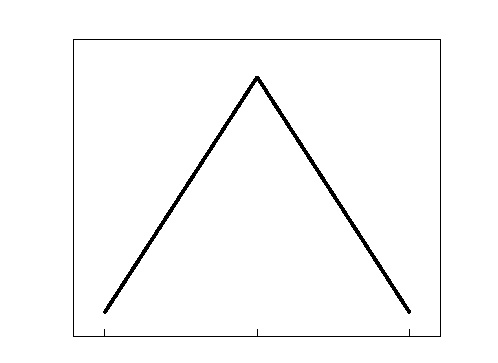
\includegraphics[width={223.20bp},height={158.40bp}]{pocatecni_rozlozeni_teploty}}%
    \gplfronttext
  \end{picture}%
\endgroup

  \caption{Počáteční rozložení teploty ve vzorku}
\end{figure}
 
\section{Teorie}

Obecně se vedení tepla v jednorozměrném systému řídí rovnicí

\begin{equation}
\frac{\partial t(x, \tau)}{\partial \tau} = \frac{\lambda}{\rho c} \frac{\partial^2 t(x,r)}{\partial x^2},
\end{equation}

\noindent
kde $\lambda$ je součinitel tepelné vodivosti, t teplota,  $\tau$ čas, x souřadnice ve vzorku, c tepelná kapacita a $\rho$ hustota materiálu v bodě x. Celý výraz $\frac{\lambda}{\rho c}$ se navíc nazývá teplotní vodivost. Je jedinou veličinou, která závisí na materiálu vzorku a tím i jedinou veličinou která určuje jak se mění rozložení teploty s časem a polohou. 

Dosazením podmínek popsaných v úvodu vyhovuje rovnici 1 analytický vztah

\begin{equation}
  t(x, \tau) = t_0 + \sum_{n=1, n \text{ liché}}^{\infty} \frac{8(t_{max} - t_0)}{\pi^2 n^2}\cos(\frac{\pi n x}{l})\exp(- \frac{\lambda}{\rho c} (\frac{\pi n}{l})^2 \tau), 
\end{equation}

\noindent
kde $t_0$ je konstantní teplota na okrajích, $t_{max}$ počáteční hodnota uprostřed a l délka vzorku.

Jednotlivé členy nekonečné sumy jsou nepřímo úměrné $n^2$ a zároveň mají $-n^2$ v exponentu. Můžeme tedy očekávat, že příspěvek 1. členu budu s časem stále více dominantní. Když navíc dosadíme za x=0 pro střed vzorku, dostaneme aproximativní vztah

\begin{equation}
  t(\tau) = t_0 + \frac{8(t_{max} - t_0)}{\pi^2}\exp(- \frac{\lambda}{\rho c} (\frac{\pi}{l})^2 \tau).
\end{equation}

\begin{figure}[htpb]
  \centering
  % GNUPLOT: LaTeX picture with Postscript
\begingroup
  \makeatletter
  \providecommand\color[2][]{%
    \GenericError{(gnuplot) \space\space\space\@spaces}{%
      Package color not loaded in conjunction with
      terminal option `colourtext'%
    }{See the gnuplot documentation for explanation.%
    }{Either use 'blacktext' in gnuplot or load the package
      color.sty in LaTeX.}%
    \renewcommand\color[2][]{}%
  }%
  \providecommand\includegraphics[2][]{%
    \GenericError{(gnuplot) \space\space\space\@spaces}{%
      Package graphicx or graphics not loaded%
    }{See the gnuplot documentation for explanation.%
    }{The gnuplot epslatex terminal needs graphicx.sty or graphics.sty.}%
    \renewcommand\includegraphics[2][]{}%
  }%
  \providecommand\rotatebox[2]{#2}%
  \@ifundefined{ifGPcolor}{%
    \newif\ifGPcolor
    \GPcolorfalse
  }{}%
  \@ifundefined{ifGPblacktext}{%
    \newif\ifGPblacktext
    \GPblacktexttrue
  }{}%
  % define a \g@addto@macro without @ in the name:
  \let\gplgaddtomacro\g@addto@macro
  % define empty templates for all commands taking text:
  \gdef\gplbacktext{}%
  \gdef\gplfronttext{}%
  \makeatother
  \ifGPblacktext
    % no textcolor at all
    \def\colorrgb#1{}%
    \def\colorgray#1{}%
  \else
    % gray or color?
    \ifGPcolor
      \def\colorrgb#1{\color[rgb]{#1}}%
      \def\colorgray#1{\color[gray]{#1}}%
      \expandafter\def\csname LTw\endcsname{\color{white}}%
      \expandafter\def\csname LTb\endcsname{\color{black}}%
      \expandafter\def\csname LTa\endcsname{\color{black}}%
      \expandafter\def\csname LT0\endcsname{\color[rgb]{1,0,0}}%
      \expandafter\def\csname LT1\endcsname{\color[rgb]{0,1,0}}%
      \expandafter\def\csname LT2\endcsname{\color[rgb]{0,0,1}}%
      \expandafter\def\csname LT3\endcsname{\color[rgb]{1,0,1}}%
      \expandafter\def\csname LT4\endcsname{\color[rgb]{0,1,1}}%
      \expandafter\def\csname LT5\endcsname{\color[rgb]{1,1,0}}%
      \expandafter\def\csname LT6\endcsname{\color[rgb]{0,0,0}}%
      \expandafter\def\csname LT7\endcsname{\color[rgb]{1,0.3,0}}%
      \expandafter\def\csname LT8\endcsname{\color[rgb]{0.5,0.5,0.5}}%
    \else
      % gray
      \def\colorrgb#1{\color{black}}%
      \def\colorgray#1{\color[gray]{#1}}%
      \expandafter\def\csname LTw\endcsname{\color{white}}%
      \expandafter\def\csname LTb\endcsname{\color{black}}%
      \expandafter\def\csname LTa\endcsname{\color{black}}%
      \expandafter\def\csname LT0\endcsname{\color{black}}%
      \expandafter\def\csname LT1\endcsname{\color{black}}%
      \expandafter\def\csname LT2\endcsname{\color{black}}%
      \expandafter\def\csname LT3\endcsname{\color{black}}%
      \expandafter\def\csname LT4\endcsname{\color{black}}%
      \expandafter\def\csname LT5\endcsname{\color{black}}%
      \expandafter\def\csname LT6\endcsname{\color{black}}%
      \expandafter\def\csname LT7\endcsname{\color{black}}%
      \expandafter\def\csname LT8\endcsname{\color{black}}%
    \fi
  \fi
    \setlength{\unitlength}{0.0500bp}%
    \ifx\gptboxheight\undefined%
      \newlength{\gptboxheight}%
      \newlength{\gptboxwidth}%
      \newsavebox{\gptboxtext}%
    \fi%
    \setlength{\fboxrule}{0.5pt}%
    \setlength{\fboxsep}{1pt}%
    \definecolor{tbcol}{rgb}{1,1,1}%
\begin{picture}(7200.00,3600.00)%
    \gplgaddtomacro\gplbacktext{%
      \csname LTb\endcsname%%
      \put(1818,364){\makebox(0,0)[r]{\strut{}$0$}}%
      \put(1818,875){\makebox(0,0)[r]{\strut{}$20$}}%
      \put(1818,1386){\makebox(0,0)[r]{\strut{}$40$}}%
      \put(1818,1897){\makebox(0,0)[r]{\strut{}$60$}}%
      \put(1818,2408){\makebox(0,0)[r]{\strut{}$80$}}%
      \put(1818,2919){\makebox(0,0)[r]{\strut{}$100$}}%
      \put(2125,-112){\makebox(0,0){\strut{}$-0.5$}}%
      \put(3875,-112){\makebox(0,0){\strut{}$0$}}%
      \put(5624,-112){\makebox(0,0){\strut{}$0.5$}}%
    }%
    \gplgaddtomacro\gplfronttext{%
      \csname LTb\endcsname%%
      \put(5819,3065){\makebox(0,0)[r]{\strut{}0 min}}%
      \csname LTb\endcsname%%
      \put(5819,2845){\makebox(0,0)[r]{\strut{}2 min}}%
      \csname LTb\endcsname%%
      \put(5819,2625){\makebox(0,0)[r]{\strut{}5 min}}%
      \csname LTb\endcsname%%
      \put(5819,2405){\makebox(0,0)[r]{\strut{}10 min}}%
      \csname LTb\endcsname%%
      \put(5819,2185){\makebox(0,0)[r]{\strut{}20 min}}%
      \csname LTb\endcsname%%
      \put(1213,1743){\rotatebox{-270.00}{\makebox(0,0){\strut{}teplota $^{\circ}$ C}}}%
      \put(3874,-442){\makebox(0,0){\strut{}x / m}}%
    }%
    \gplbacktext
    \put(0,0){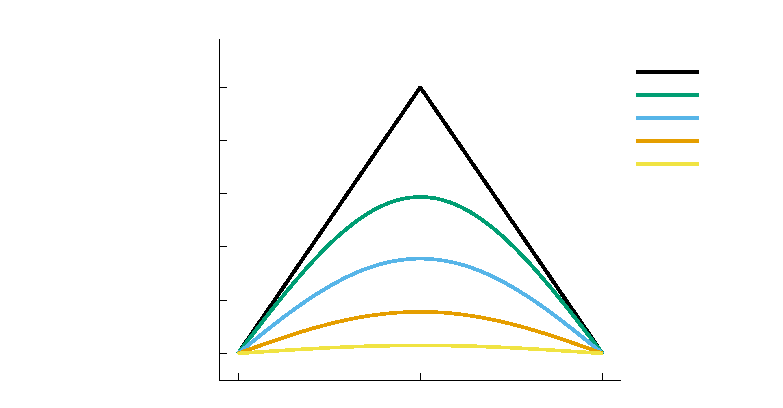
\includegraphics[width={360.00bp},height={180.00bp}]{casovy_vyvoj_teploty}}%
    \gplfronttext
  \end{picture}%
\endgroup

  \caption{Závislost rozložení teploty $t(x, \tau)$ ve vzorku pro $\frac{\lambda}{\rho c}$ = 3.6 $\cdot$ 10$^{-3}$ m$^2$ s$^{-1}$}
\end{figure}


\begin{figure}[htpb]
  \centering
  % GNUPLOT: LaTeX picture with Postscript
\begingroup
  \makeatletter
  \providecommand\color[2][]{%
    \GenericError{(gnuplot) \space\space\space\@spaces}{%
      Package color not loaded in conjunction with
      terminal option `colourtext'%
    }{See the gnuplot documentation for explanation.%
    }{Either use 'blacktext' in gnuplot or load the package
      color.sty in LaTeX.}%
    \renewcommand\color[2][]{}%
  }%
  \providecommand\includegraphics[2][]{%
    \GenericError{(gnuplot) \space\space\space\@spaces}{%
      Package graphicx or graphics not loaded%
    }{See the gnuplot documentation for explanation.%
    }{The gnuplot epslatex terminal needs graphicx.sty or graphics.sty.}%
    \renewcommand\includegraphics[2][]{}%
  }%
  \providecommand\rotatebox[2]{#2}%
  \@ifundefined{ifGPcolor}{%
    \newif\ifGPcolor
    \GPcolorfalse
  }{}%
  \@ifundefined{ifGPblacktext}{%
    \newif\ifGPblacktext
    \GPblacktexttrue
  }{}%
  % define a \g@addto@macro without @ in the name:
  \let\gplgaddtomacro\g@addto@macro
  % define empty templates for all commands taking text:
  \gdef\gplbacktext{}%
  \gdef\gplfronttext{}%
  \makeatother
  \ifGPblacktext
    % no textcolor at all
    \def\colorrgb#1{}%
    \def\colorgray#1{}%
  \else
    % gray or color?
    \ifGPcolor
      \def\colorrgb#1{\color[rgb]{#1}}%
      \def\colorgray#1{\color[gray]{#1}}%
      \expandafter\def\csname LTw\endcsname{\color{white}}%
      \expandafter\def\csname LTb\endcsname{\color{black}}%
      \expandafter\def\csname LTa\endcsname{\color{black}}%
      \expandafter\def\csname LT0\endcsname{\color[rgb]{1,0,0}}%
      \expandafter\def\csname LT1\endcsname{\color[rgb]{0,1,0}}%
      \expandafter\def\csname LT2\endcsname{\color[rgb]{0,0,1}}%
      \expandafter\def\csname LT3\endcsname{\color[rgb]{1,0,1}}%
      \expandafter\def\csname LT4\endcsname{\color[rgb]{0,1,1}}%
      \expandafter\def\csname LT5\endcsname{\color[rgb]{1,1,0}}%
      \expandafter\def\csname LT6\endcsname{\color[rgb]{0,0,0}}%
      \expandafter\def\csname LT7\endcsname{\color[rgb]{1,0.3,0}}%
      \expandafter\def\csname LT8\endcsname{\color[rgb]{0.5,0.5,0.5}}%
    \else
      % gray
      \def\colorrgb#1{\color{black}}%
      \def\colorgray#1{\color[gray]{#1}}%
      \expandafter\def\csname LTw\endcsname{\color{white}}%
      \expandafter\def\csname LTb\endcsname{\color{black}}%
      \expandafter\def\csname LTa\endcsname{\color{black}}%
      \expandafter\def\csname LT0\endcsname{\color{black}}%
      \expandafter\def\csname LT1\endcsname{\color{black}}%
      \expandafter\def\csname LT2\endcsname{\color{black}}%
      \expandafter\def\csname LT3\endcsname{\color{black}}%
      \expandafter\def\csname LT4\endcsname{\color{black}}%
      \expandafter\def\csname LT5\endcsname{\color{black}}%
      \expandafter\def\csname LT6\endcsname{\color{black}}%
      \expandafter\def\csname LT7\endcsname{\color{black}}%
      \expandafter\def\csname LT8\endcsname{\color{black}}%
    \fi
  \fi
    \setlength{\unitlength}{0.0500bp}%
    \ifx\gptboxheight\undefined%
      \newlength{\gptboxheight}%
      \newlength{\gptboxwidth}%
      \newsavebox{\gptboxtext}%
    \fi%
    \setlength{\fboxrule}{0.5pt}%
    \setlength{\fboxsep}{1pt}%
    \definecolor{tbcol}{rgb}{1,1,1}%
\begin{picture}(5760.00,3600.00)%
    \gplgaddtomacro\gplbacktext{%
      \csname LTb\endcsname%%
      \put(814,1394){\makebox(0,0)[r]{\strut{}$10$}}%
      \put(814,3233){\makebox(0,0)[r]{\strut{}$100$}}%
      \put(1348,-112){\makebox(0,0){\strut{}$0$}}%
      \put(2351,-112){\makebox(0,0){\strut{}$5$}}%
      \put(3355,-112){\makebox(0,0){\strut{}$10$}}%
      \put(4359,-112){\makebox(0,0){\strut{}$15$}}%
      \put(5363,-112){\makebox(0,0){\strut{}$20$}}%
    }%
    \gplgaddtomacro\gplfronttext{%
      \csname LTb\endcsname%%
      \put(4376,3206){\makebox(0,0)[r]{\strut{}approx}}%
      \csname LTb\endcsname%%
      \put(209,1743){\rotatebox{-270.00}{\makebox(0,0){\strut{}teplota $^{\circ}$ C}}}%
      \put(3154,-442){\makebox(0,0){\strut{}$\tau$ min}}%
    }%
    \gplbacktext
    \put(0,0){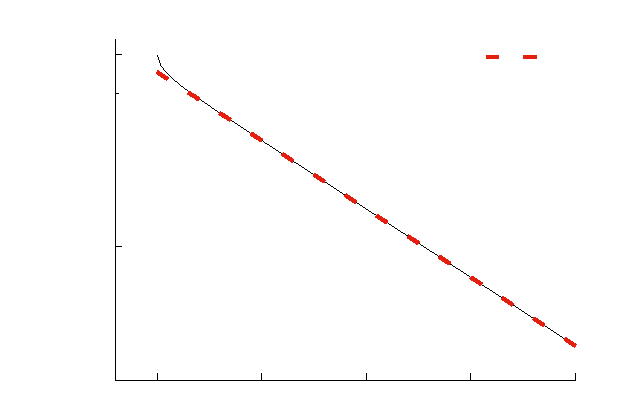
\includegraphics[width={288.00bp},height={180.00bp}]{casovy_vyvoj_teploty_uprostred}}%
    \gplfronttext
  \end{picture}%
\endgroup

  \caption{Závislost teploty ve středu vzorku na čase v logaritmické stupnici.}
\end{figure}

\section{Postup měření}

Nejprve je potřeba zajistit rozložení teploty z grafu 1. Víme, že pokud se teplo šíří přímo od ohřívače k chladiči o stálých teplotách bez ztrát do okolí, bude rozložení teploty na této přímce lineární. Nejjednodušší je celou soustavu udělat mnohem širší než vysokou, což uprostřed napodobuje případ nekonečných rozměrů, kde není ani okolí ani nejsou ztráty do okolí.

K dispozici mám 2 chladiče, topnou fólii a sádrokartonové desky jako vzorek. Na chladič položím sádrokarton, pak topnou fólii, další desku a nahoru druhý chladič. Sádrokartonové desky mají navíc na obou stranách vyhloubené drážky, kudy se dá protáhnout teplotní čidlo až doprostřed. Čidla budou tedy 4 umístěné z obou stran obou desek. 

\section{Výsledky měření}

Určil jsem rozměry a hmotnost čtvercové sádrokartonové desky na
\begin{align*}
  \frac{l}{2} = (1.26 \pm 0.03) \text{ cm} \\
  a = (20.0 \pm 0.4) \text{ cm} \\
  m = (379.4 \pm 2) \text{ g.} \\
\end{align*}

Dopočítaná hustota je $\rho$ = (750 $\pm$ 30) kg m$^3$ a měrnou tepelnou kapacitu c = 1100 J Kg$^{-1}$ K$^{-1}$ jsem našel v tabulkách.


\begin{figure}[htpb]
  \centering
  % GNUPLOT: LaTeX picture with Postscript
\begingroup
  \makeatletter
  \providecommand\color[2][]{%
    \GenericError{(gnuplot) \space\space\space\@spaces}{%
      Package color not loaded in conjunction with
      terminal option `colourtext'%
    }{See the gnuplot documentation for explanation.%
    }{Either use 'blacktext' in gnuplot or load the package
      color.sty in LaTeX.}%
    \renewcommand\color[2][]{}%
  }%
  \providecommand\includegraphics[2][]{%
    \GenericError{(gnuplot) \space\space\space\@spaces}{%
      Package graphicx or graphics not loaded%
    }{See the gnuplot documentation for explanation.%
    }{The gnuplot epslatex terminal needs graphicx.sty or graphics.sty.}%
    \renewcommand\includegraphics[2][]{}%
  }%
  \providecommand\rotatebox[2]{#2}%
  \@ifundefined{ifGPcolor}{%
    \newif\ifGPcolor
    \GPcolorfalse
  }{}%
  \@ifundefined{ifGPblacktext}{%
    \newif\ifGPblacktext
    \GPblacktexttrue
  }{}%
  % define a \g@addto@macro without @ in the name:
  \let\gplgaddtomacro\g@addto@macro
  % define empty templates for all commands taking text:
  \gdef\gplbacktext{}%
  \gdef\gplfronttext{}%
  \makeatother
  \ifGPblacktext
    % no textcolor at all
    \def\colorrgb#1{}%
    \def\colorgray#1{}%
  \else
    % gray or color?
    \ifGPcolor
      \def\colorrgb#1{\color[rgb]{#1}}%
      \def\colorgray#1{\color[gray]{#1}}%
      \expandafter\def\csname LTw\endcsname{\color{white}}%
      \expandafter\def\csname LTb\endcsname{\color{black}}%
      \expandafter\def\csname LTa\endcsname{\color{black}}%
      \expandafter\def\csname LT0\endcsname{\color[rgb]{1,0,0}}%
      \expandafter\def\csname LT1\endcsname{\color[rgb]{0,1,0}}%
      \expandafter\def\csname LT2\endcsname{\color[rgb]{0,0,1}}%
      \expandafter\def\csname LT3\endcsname{\color[rgb]{1,0,1}}%
      \expandafter\def\csname LT4\endcsname{\color[rgb]{0,1,1}}%
      \expandafter\def\csname LT5\endcsname{\color[rgb]{1,1,0}}%
      \expandafter\def\csname LT6\endcsname{\color[rgb]{0,0,0}}%
      \expandafter\def\csname LT7\endcsname{\color[rgb]{1,0.3,0}}%
      \expandafter\def\csname LT8\endcsname{\color[rgb]{0.5,0.5,0.5}}%
    \else
      % gray
      \def\colorrgb#1{\color{black}}%
      \def\colorgray#1{\color[gray]{#1}}%
      \expandafter\def\csname LTw\endcsname{\color{white}}%
      \expandafter\def\csname LTb\endcsname{\color{black}}%
      \expandafter\def\csname LTa\endcsname{\color{black}}%
      \expandafter\def\csname LT0\endcsname{\color{black}}%
      \expandafter\def\csname LT1\endcsname{\color{black}}%
      \expandafter\def\csname LT2\endcsname{\color{black}}%
      \expandafter\def\csname LT3\endcsname{\color{black}}%
      \expandafter\def\csname LT4\endcsname{\color{black}}%
      \expandafter\def\csname LT5\endcsname{\color{black}}%
      \expandafter\def\csname LT6\endcsname{\color{black}}%
      \expandafter\def\csname LT7\endcsname{\color{black}}%
      \expandafter\def\csname LT8\endcsname{\color{black}}%
    \fi
  \fi
    \setlength{\unitlength}{0.0500bp}%
    \ifx\gptboxheight\undefined%
      \newlength{\gptboxheight}%
      \newlength{\gptboxwidth}%
      \newsavebox{\gptboxtext}%
    \fi%
    \setlength{\fboxrule}{0.5pt}%
    \setlength{\fboxsep}{1pt}%
    \definecolor{tbcol}{rgb}{1,1,1}%
\begin{picture}(8640.00,5040.00)%
    \gplgaddtomacro\gplbacktext{%
      \csname LTb\endcsname%%
      \put(682,151){\makebox(0,0)[r]{\strut{}$10$}}%
      \put(682,929){\makebox(0,0)[r]{\strut{}$20$}}%
      \put(682,1707){\makebox(0,0)[r]{\strut{}$30$}}%
      \put(682,2485){\makebox(0,0)[r]{\strut{}$40$}}%
      \put(682,3263){\makebox(0,0)[r]{\strut{}$50$}}%
      \put(682,4041){\makebox(0,0)[r]{\strut{}$60$}}%
      \put(682,4819){\makebox(0,0)[r]{\strut{}$70$}}%
      \put(1726,-69){\makebox(0,0){\strut{}$2000$}}%
      \put(2812,-69){\makebox(0,0){\strut{}$2500$}}%
      \put(3899,-69){\makebox(0,0){\strut{}$3000$}}%
      \put(4985,-69){\makebox(0,0){\strut{}$3500$}}%
      \put(6071,-69){\makebox(0,0){\strut{}$4000$}}%
      \put(7157,-69){\makebox(0,0){\strut{}$4500$}}%
      \put(8243,-69){\makebox(0,0){\strut{}$5000$}}%
    }%
    \gplgaddtomacro\gplfronttext{%
      \csname LTb\endcsname%%
      \put(7256,4646){\makebox(0,0)[r]{\strut{}čidlo 1}}%
      \csname LTb\endcsname%%
      \put(7256,4426){\makebox(0,0)[r]{\strut{}čidlo 2}}%
      \csname LTb\endcsname%%
      \put(7256,4206){\makebox(0,0)[r]{\strut{}čidlo 3}}%
      \csname LTb\endcsname%%
      \put(7256,3986){\makebox(0,0)[r]{\strut{}čidlo 4}}%
      \csname LTb\endcsname%%
      \put(7256,3766){\makebox(0,0)[r]{\strut{}fit}}%
      \csname LTb\endcsname%%
      \put(209,2485){\rotatebox{-270.00}{\makebox(0,0){\strut{}t $^{\circ} C$}}}%
      \put(4528,-399){\makebox(0,0){\strut{}$\tau$ [s]}}%
    }%
    \gplbacktext
    \put(0,0){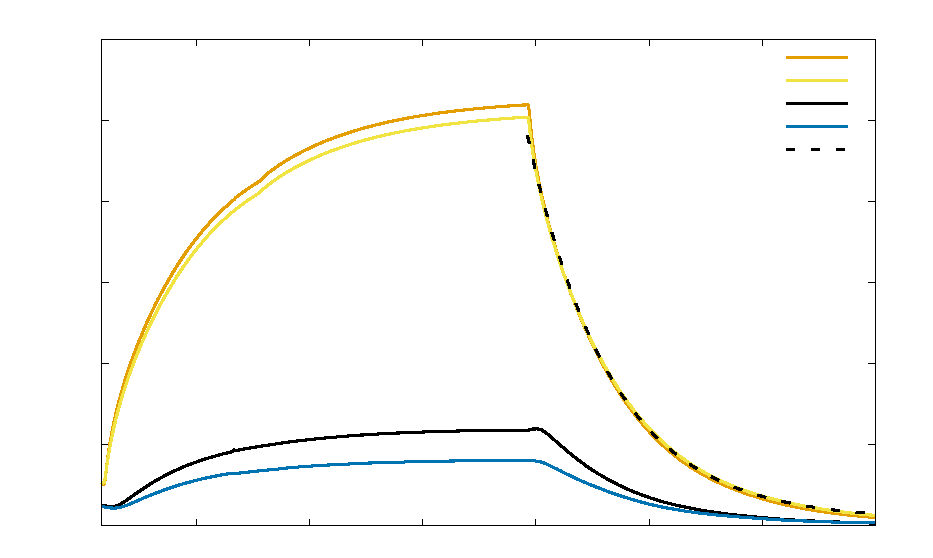
\includegraphics[width={432.00bp},height={252.00bp}]{mereni}}%
    \gplfronttext
  \end{picture}%
\endgroup

  \caption{Závislost teploty na čase uprostřed a na krajích vzorku }
  \caption*{$\lambda$ = (0.143 $\pm$ 0.009) W m$^{-1}$ K$^{-1}$}
\end{figure}

\section{Závěr}

Pomocí realizace analytického řešení (3) rovnice vedení tepla jsem změřil součinitel tepelné vodivosti sádrokartonu $\lambda$=(0.143 $\pm$ 0.009) W m$^{-1}$ K$^{-1}$. Tabulková hodnota z odkazu 1 je 0.220~W~m$^{-1}$~K$^{-1}$. Největším příspěvkem chyby mého výsledku je pravděpodobně nedostatečně výkonný chladič. Konce tyče, které měly mít stabilní teplotu, se, jak je vidět v grafu 4, pohybovaly na intervalu asi 10 $^{\circ}$C. Stálá počáteční teplota $t_0$=20 $^{\circ}$C by vedla k rychlejšímu chladnutí, strmějšímu grafu a vyšší tepelné vodivosti. Přesto je fit exponencielou velmi přesný kromě intervalu kolem času $t_0$, což odpovídá teorii. 

\begin{thebibliography}{0}
\bibitem{tabulky} Katalog stavebních materiálů ~\url{https://stavba.tzb-info.cz/docu/tabulky/0000/000086_katalog.html}.   
\end{thebibliography}

\end{document}
